% Chapter Template

\chapter{Introduction} % Main chapter title

\label{Chapter1} % Change X to a consecutive number; for referencing this chapter elsewhere, use \ref{ChapterX}

\lhead{Chapter 1. \emph{Introduction}} % Change X to a consecutive number; this is for the header on each page - perhaps a shortened title

%----------------------------------------------------------------------------------------
%	SECTION 1 - Voice Activity Detection
%----------------------------------------------------------------------------------------

\section{Voice Activity Detection}

Voice Activity Detection (VAD) is a process of identifying parts of an audio recording which contain the presence of human voice as opposed to those which are only comprised of silence or the background noise. VAD is a relatively simple task in recordings which have high signal-to-noise ratios (SNR), in which voice can be distinguished from noise simply by computing the short-time energy of all frames and setting an appropriate threshold for their classification. However, in most modern applications, the signal is almost always corrupted to some extent by a background noise which makes the VAD performance to deteriorate. While some types of noise can be relatively easily dealt with, i.e. those with spectral characteristics different from speech, in the presence of other, it might be very difficult to identify speech segments. One such noise type might be the \emph{babble noise} which consists of speech that we are not interested in. Additionally, VAD decision is especially difficult for the unvoiced phonemes \cite{Kondoz} whose spectrum contains no periodicity and is often similar to the one of white noise \cite{Michaelis}.

There has been an active research in the VAD area from as early as 1975, when Rabiner and Sambur \cite{RabinerSambur} proposed a VAD algorithm (then referred to as \emph{algorithm for determining the endpoints of isolated utterances}) based on the aforementioned short-time energy and the zero-crossing rate. This approach works reasonably well for signals with the SNR on the order of 30 dB and is suitable for a variety of applications which are not subject to a constant, high level of background noise, such as Voice over IP, when a person speaks to a closely positioned microphone in a relatively calm environment. However since then there has been a need for much better performance, including algorithms whose robustness has to be achieved even at negative SNRs. A person driving a car, trying to communicate with their smartphone through its built-in speech recognition system (e.g. Apple Siri) might be one example of such application. Figure \ref{fig:corruptedSpeech} shows a comparison of the amplitude of a clean utterance with the same utterance corrupted by a -5 dB car noise. As it can be seen, some parts of the recording are completely submerged in the noise (especially during the second second of the recording) and their detection poses a considerable challenge for any VAD system. In robotics there is often a desire to communicate with the robot by speaking from a distance which naturally decreases power of the received signal. Taking the detrimental effect of the background noise into consideration, the simple algorithms are likely to either fail completely or their performance might significantly drop.

\begin{figure}[htbp]
	\centering
		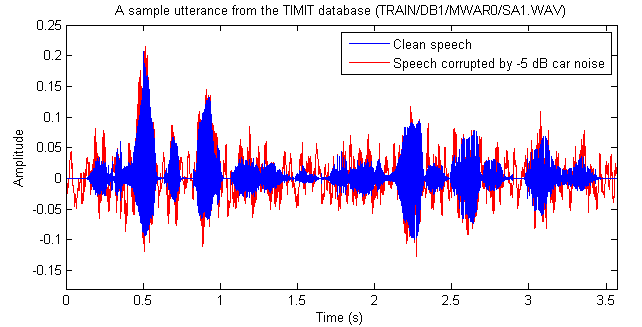
\includegraphics[width=0.9\columnwidth]{Figures/corruptedSpeech.png}
		\rule{37em}{0.5pt}
	\caption[A sample utterance corrupted by -5 dB car noise]{A sample utterance from the TIMIT speech corpus corrupted by -5 dB car noise from the NOISEX-92 database}
	\label{fig:corruptedSpeech}
\end{figure}

%Recently, numerous VAD approaches have been proposed, based on various features such as ..... ..... ..... . 

%----------------------------------------------------------------------------------------
%	SECTION 2 - Applications of VAD 
%----------------------------------------------------------------------------------------

\section{Applications of VAD}

VAD is often the first step in many signal processing applications including speech recognition \cite{RamirezGorriz, Kuroiwa, Martin, Shafran, ImprovedLikelihood, LTSD}, speech coding and transmission \cite{Sohn, RamirezGorriz, Prasad, G729, GSMControl}, speech enhancement \cite{Park, RamirezGorriz, Borisagar}, noise estimation \cite{RamirezGorriz} or speaker recognition \cite{Sahidullah}. In most applications the noise-robust VAD decisions reduce the computational load required by the system and improve its accuracy. The reduced computational load is achieved since the voice-inactive frames are often either transmitted at a much lower bit-rate or not processed at all. At the same time, the clear boundaries of an utterance help to improve the accuracy of some systems (e.g. speech recognition).

\subsection{Automatic Speech Recognition}

In Automatic Speech Recognition (ASR), it is of importance to first extract the voice-active parts of a signal which can then be passed to the actual recognition module. This procedure increases both the accuracy of the ASR system as well as its speed, since the recognition task is not performed on the parts of the signal which do not contain speech. A sample block diagram of an ASR system which uses a VAD module is presented in Figure \ref{fig:ASRVAD} \cite{RamirezGorriz}. For ASR, and also most other applications, it is crucial for the VAD module to be able to identify all speech segments in order not to degrade the accuracy of the entire system. Therefore, VAD systems often implement a fail-safe approach which means that if there is an uncertainty in classification of a frame, it is safer to label is as speech than otherwise. Typically, there is a trade-off in VAD performance which can be characterised as maximising the precision while keeping the recall at a steady, high rate.

\begin{figure}[htbp]
	\centering
		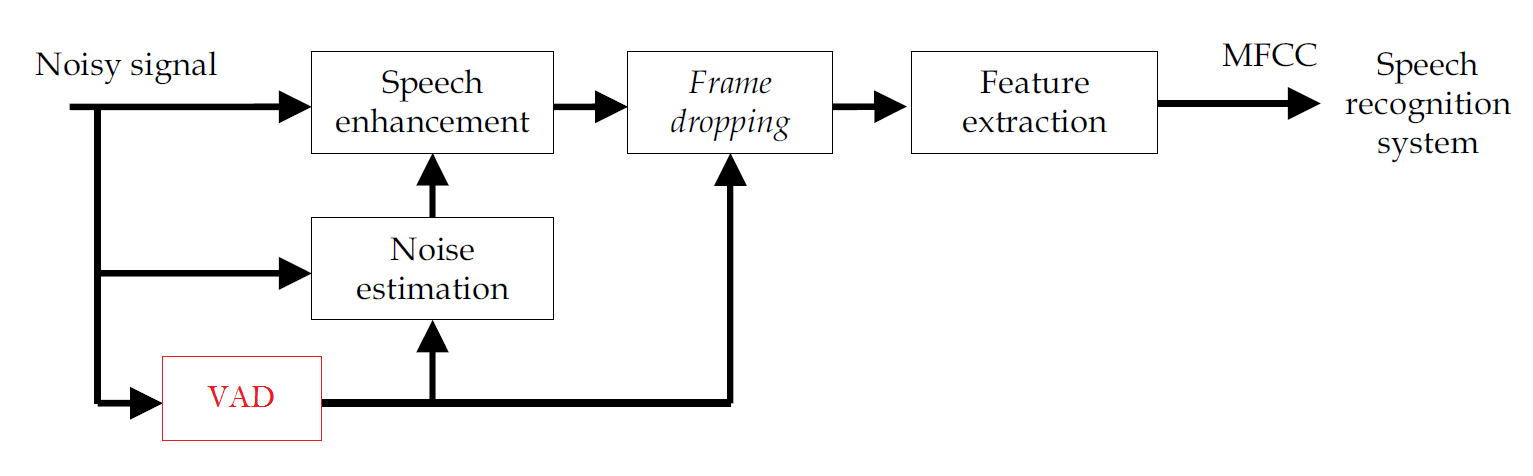
\includegraphics[width=1\columnwidth]{Figures/ASRVAD.png}
		\rule{37em}{0.5pt}
	\caption[Automatic Speech Recognition system with Voice Activity Detection module]{Block diagram of an Automatic Speech Recognition system with Voice Activity Detection module \cite{RamirezGorriz}}
	\label{fig:ASRVAD}
\end{figure}

\subsection{Speech Coding and Transmission}

A typical phone conversation involves each person speaking on average no more than 50\% of the time \citep{GSMControl}. From this fact it can be concluded that signal transmission would be greatly optimised if each transmitter was switched-off half of the time. Such approach could cause the overall system capacity to double. The technique of interrupted transmission during periods of silence is known as discontinuous transmission (DTX). In order to work properly, it requires a precise Voice Activity Detection to direct the operation of a transmitter between being switched on or off. As an alternate method to stopping the transmission, a dual-mode encoding technique could be employed, which uses a higher bit-rate for coding the voice-active frames and lower for silence/noise. The latter is precisely what the popular ITU-T G.729 Annex B \cite{G729} standard does, transmitting the voice-active parts at a fixed bit rate of 8 kb/s while the noisy ones at only 15 b/frame.

Figure \ref{fig:DTXVAD} shows a high-level structure of a dual-mode coding and transmission system, in which the VAD module is used to direct the incoming signal into either the active or inactive speech encoder. The noise can be either transmitted at a much lower bit-rate or the transmission might be switched off completely. In case of a stopped transmission, the receiving end often implements a \emph{comfort noise} \citep{GSMControl,G729,RamirezGorriz} generation module, which creates a synthetic signal similar to the background noise at the transmitter so that the listener does not notice the rapid, inconvenient switching during the conversation.

\begin{figure}[htbp]
	\centering
		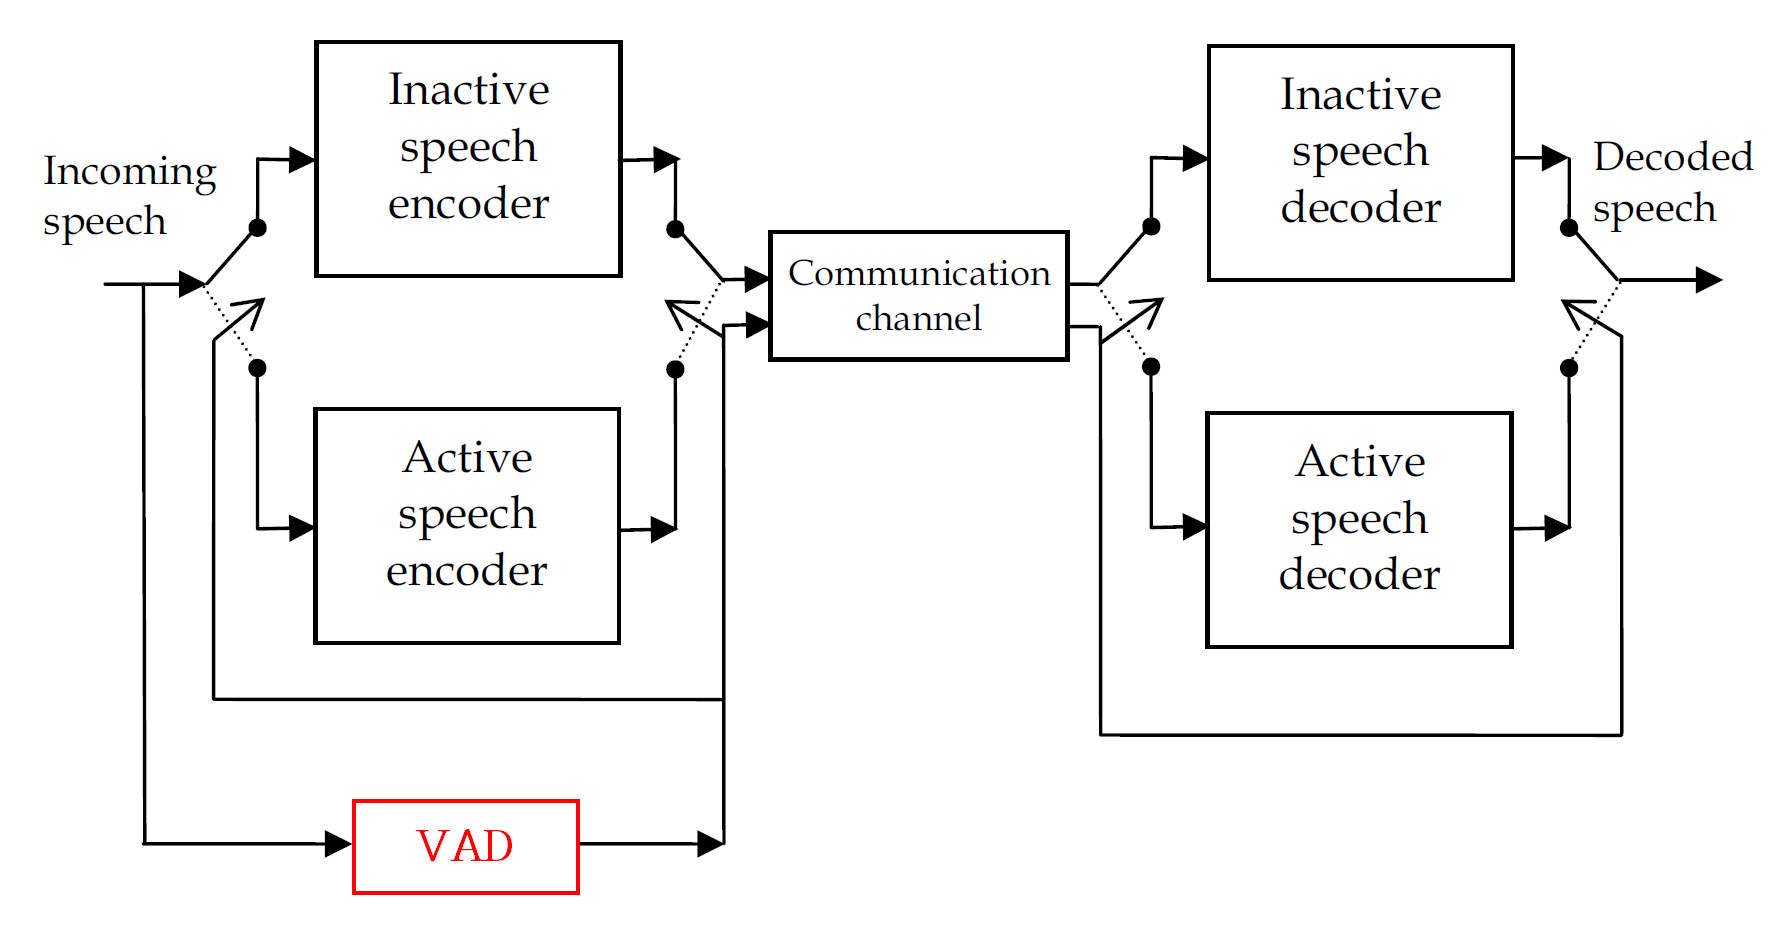
\includegraphics[width=1\columnwidth]{Figures/DTXVAD.png}
		\rule{37em}{0.5pt}
	\caption[Dual-mode transmission system with Voice Activity Detection module]{Block diagram of an dual-mode transmission system with Voice Activity Detection module \cite{G729}}
	\label{fig:DTXVAD}
\end{figure}

\subsection{Noise Estimation and Speech Enhancement}

Speech enhancement aims to improve the intelligibility and quality of speech signals corrupted by additive  noise of some kind. Many speech enhancement systems use a technique called \emph{spectral subtraction} \cite{Kondoz, RamirezGorriz}. It assumes, that the clean speech can be represented in the frequency-domain in the form:
\begin{equation}
|S(f)| = |Y(f)| - |N(f)|
\end{equation}
where $|Y(f)|$ is the amplitude spectrum of the corrupted speech, $|S(f)|$ of the clean speech and $|N(f)|$ of the noise. In order for this technique to work, the noise needs to be additive, stationary and uncorrelated with the clean speech signal. Additionally, one needs to estimate the spectrum of the noise, which in real-world applications where a variety of different, often nonstationary, noise types are encountered, is a nontrivial problem. A robust Voice Activity Detector can become very useful in this task by identifying the voice-inactive frames of a signal from which the noise statistics could be estimated. A precise VAD can also become useful in applications dealing with slowly varying piecewise stationary noises, where the noise statistics can be adaptively estimated based on the most recent VAD decisions.

\subsection{Summary}

%----------------------------------------------------------------------------------------
%	SECTION 3 - Structure of a typical VAD system
%----------------------------------------------------------------------------------------

\section{Structure of a typical VAD system}

Figure \ref{fig:VADStructure} shows a high-level structure of a Voice Activity Detector, however only the two middle blocks are considered a core of a typical VAD system.

\begin{figure}[htbp]
	\centering
		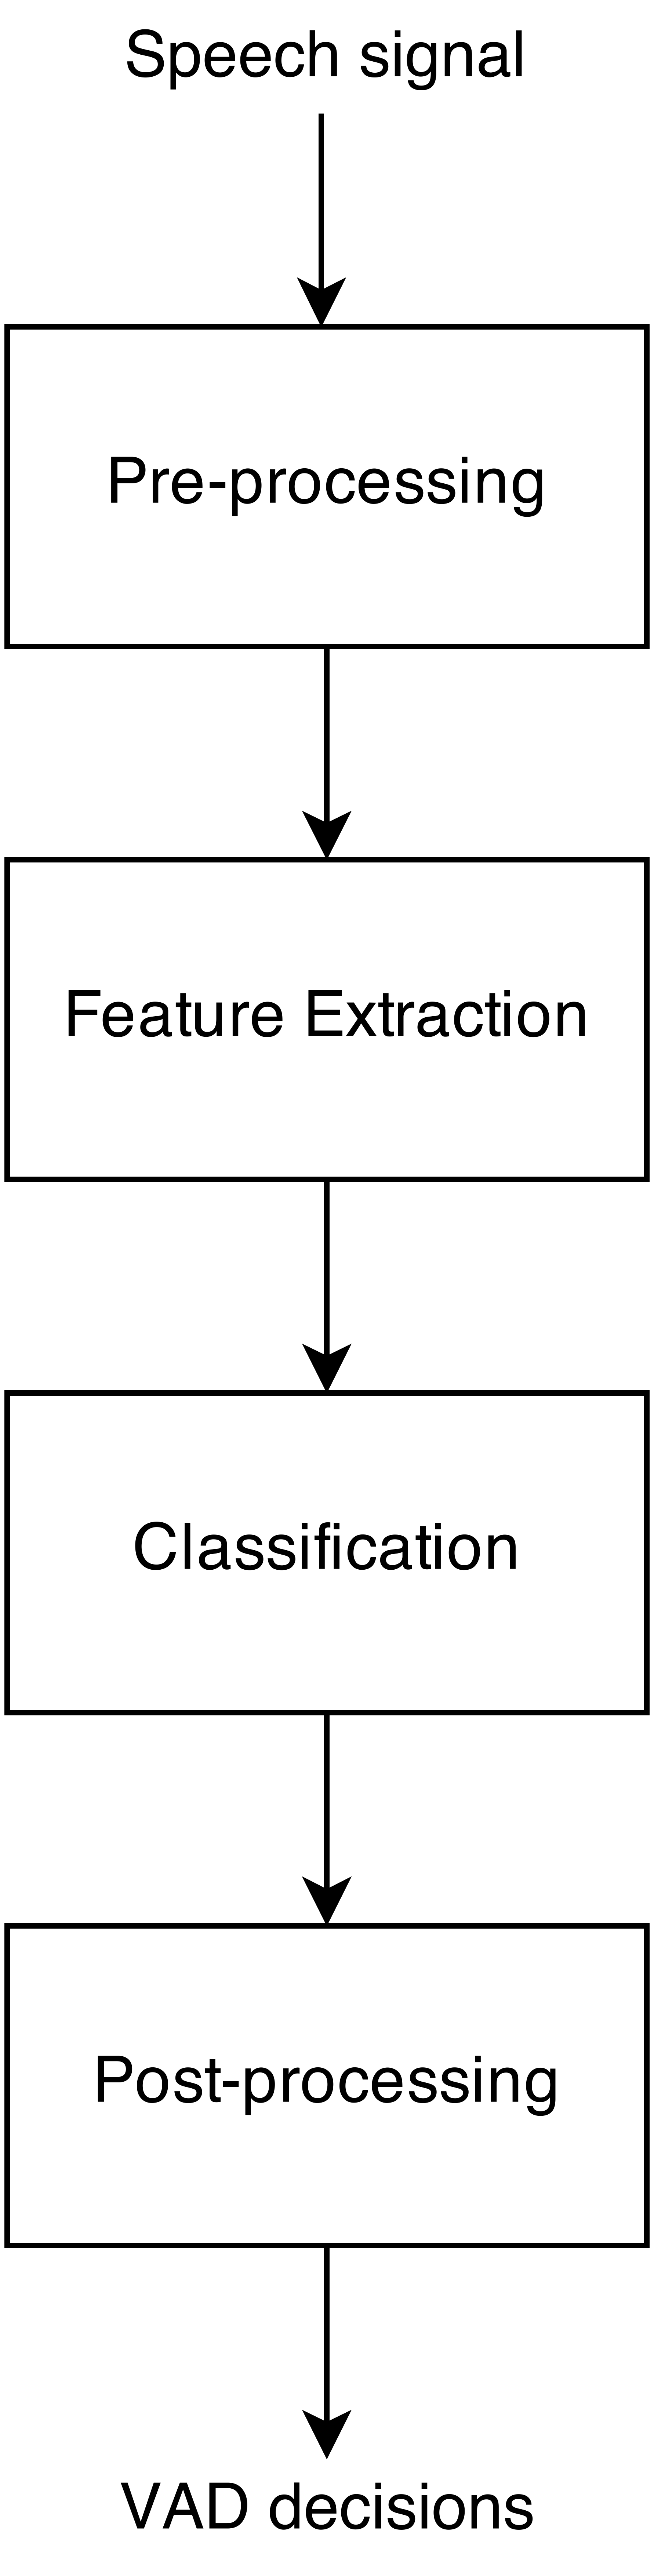
\includegraphics[width=0.15\columnwidth]{Figures/VADStructure2.png}
		\rule{37em}{0.5pt}
	\caption[Block diagram of a typical Voice Activity Detection system]{Block diagram of a typical Voice Activity Detection system}
	\label{fig:VADStructure}
\end{figure}

\subsection{Pre-processing}

The noisy speech signal is first passed to a pre-processing module which might perform a variety of tasks before the actual voice detection takes place. The module might perform noise estimation and suppression in the signal in order to improve performance of the VAD. Additionally, during pre-processing the input signal is often split into frames which are typically 10-50 ms long.

\subsection{Feature Extraction}

The purpose of the feature extraction module is to compute the speech features for each frame which are suitable for the speech/non-speech classification. These can be time domain \cite{Kida, Weaver}, frequency domain \cite{Tuske, LTSD, Tan, PARADE, RamirezMulti, Sohn, SohnInitial, Renevey}, cepstral-domain \cite{Kotcher} features or other, depending on the specific VAD algorithm. Ideally, in order to achieve the overall VAD system robustness, the selected signal characteristics should not be easily corruptible by the background noise. Additionally, the algorithms for feature extraction should be of low computational complexity for their potential usefulness in real-time applications. The output of this module is therefore a vector $\mathbf{x}$ of features for each of the frames computed in the pre-processing stage.

\subsection{Classification}

The classification module assigns a binary class (speech/non-speech) to each frame based on the feature vector $\mathbf{x}$ received from the previous processing stage. Classification might be based on a variety of decision rules, ranging from simple thresholding \cite{G729} to more advanced methods such as statistical likelihood ratio tests \cite{Sohn, ImprovedLikelihood, SohnInitial} or machine learning \cite{XiaoLei, Stadtschnitzer}. Obviously, the classifier performance degrades with the increasing power of the background noise, therefore there is a need also at this stage for a robust decision making rule. Some researchers \cite{Kida} considered a combination of multiple decision rules in making the final classification.

\subsection{Post-processing}

The last module, post-processing, often tries to \emph{smooth} the VAD decisions (i.e. perform hanging-over) in order to reduce the number of false positives and false negatives. Smoothing is important in order to precisely detect the beginnings and endings of speech bursts, which often have much lower energy than the rest of the signal. Additionally, if among 50 consecutive frames, each of 20 ms duration, only one is classified as speech, the post-processing module might change the decision for this particular frame, since it is highly unlikely for speech to be active during such short-time window. The hang-over schemes  proposed in the literature are often based on simple heuristics \cite{G729} or other techniques such as Hidden Markov models \cite{Sohn}.

%----------------------------------------------------------------------------------------
%	SECTION 4 - Thesis organisation
%----------------------------------------------------------------------------------------

\section{Thesis organisation}

The rest of this document is organised as follows:
\begin{itemize}
\item Chapter 2 contains a literature survey of both the standardised as well as recently proposed VAD algorithms from various sources such as conference proceedings or scientific journals
\item Chapter 3 presents an evaluation of selected VAD algorithms from Chapter 2 on the TIMIT speech corpus corrupted by various noise types from the NOISEX-92 database
\item 
\end{itemize}